

\tikzset{every picture/.style={line width=0.75pt}} %set default line width to 0.75pt        

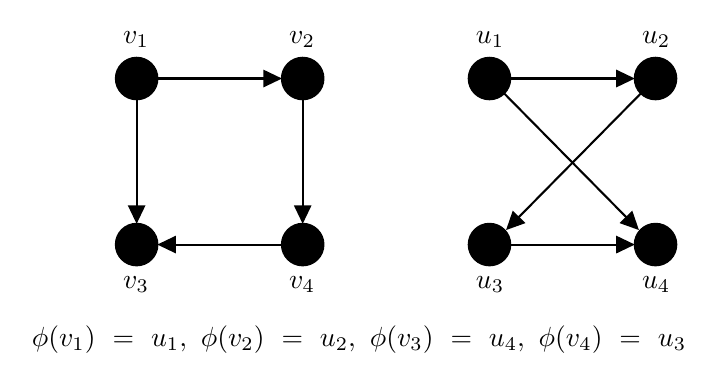
\begin{tikzpicture}[x=0.75pt,y=0.75pt,yscale=-1,xscale=1]
%uncomment if require: \path (0,184); %set diagram left start at 0, and has height of 184

%Straight Lines [id:da028261783525769912] 
\draw    (80,40) -- (137,40) ;
\draw [shift={(140,40)}, rotate = 180] [fill={rgb, 255:red, 0; green, 0; blue, 0 }  ][line width=0.08]  [draw opacity=0] (8.93,-4.29) -- (0,0) -- (8.93,4.29) -- cycle    ;
%Straight Lines [id:da5868154504079766] 
\draw    (70,50) -- (70,107) ;
\draw [shift={(70,110)}, rotate = 270] [fill={rgb, 255:red, 0; green, 0; blue, 0 }  ][line width=0.08]  [draw opacity=0] (8.93,-4.29) -- (0,0) -- (8.93,4.29) -- cycle    ;
%Straight Lines [id:da924843990160408] 
\draw    (150,50) -- (150,107) ;
\draw [shift={(150,110)}, rotate = 270] [fill={rgb, 255:red, 0; green, 0; blue, 0 }  ][line width=0.08]  [draw opacity=0] (8.93,-4.29) -- (0,0) -- (8.93,4.29) -- cycle    ;
%Straight Lines [id:da5222651223841381] 
\draw    (150,120) -- (83,120) ;
\draw [shift={(80,120)}, rotate = 360] [fill={rgb, 255:red, 0; green, 0; blue, 0 }  ][line width=0.08]  [draw opacity=0] (8.93,-4.29) -- (0,0) -- (8.93,4.29) -- cycle    ;
%Straight Lines [id:da35800782746944226] 
\draw    (240,40) -- (307,40) ;
\draw [shift={(310,40)}, rotate = 180] [fill={rgb, 255:red, 0; green, 0; blue, 0 }  ][line width=0.08]  [draw opacity=0] (8.93,-4.29) -- (0,0) -- (8.93,4.29) -- cycle    ;
%Straight Lines [id:da8484709903750047] 
\draw    (320,40) -- (250.11,110.86) ;
\draw [shift={(248,113)}, rotate = 314.6] [fill={rgb, 255:red, 0; green, 0; blue, 0 }  ][line width=0.08]  [draw opacity=0] (8.93,-4.29) -- (0,0) -- (8.93,4.29) -- cycle    ;
%Straight Lines [id:da4507216096132718] 
\draw    (240,120) -- (307,120) ;
\draw [shift={(310,120)}, rotate = 180] [fill={rgb, 255:red, 0; green, 0; blue, 0 }  ][line width=0.08]  [draw opacity=0] (8.93,-4.29) -- (0,0) -- (8.93,4.29) -- cycle    ;
%Shape: Circle [id:dp21486075935828408] 
\draw  [color={rgb, 255:red, 0; green, 0; blue, 0 }  ,draw opacity=1 ][fill={rgb, 255:red, 0; green, 0; blue, 0 }  ,fill opacity=1 ] (60,40) .. controls (60,34.48) and (64.48,30) .. (70,30) .. controls (75.52,30) and (80,34.48) .. (80,40) .. controls (80,45.52) and (75.52,50) .. (70,50) .. controls (64.48,50) and (60,45.52) .. (60,40) -- cycle ;
%Shape: Circle [id:dp6701725797486138] 
\draw  [color={rgb, 255:red, 0; green, 0; blue, 0 }  ,draw opacity=1 ][fill={rgb, 255:red, 0; green, 0; blue, 0 }  ,fill opacity=1 ] (140,40) .. controls (140,34.48) and (144.48,30) .. (150,30) .. controls (155.52,30) and (160,34.48) .. (160,40) .. controls (160,45.52) and (155.52,50) .. (150,50) .. controls (144.48,50) and (140,45.52) .. (140,40) -- cycle ;
%Shape: Circle [id:dp6472973243115998] 
\draw  [color={rgb, 255:red, 0; green, 0; blue, 0 }  ,draw opacity=1 ][fill={rgb, 255:red, 0; green, 0; blue, 0 }  ,fill opacity=1 ] (60,120) .. controls (60,114.48) and (64.48,110) .. (70,110) .. controls (75.52,110) and (80,114.48) .. (80,120) .. controls (80,125.52) and (75.52,130) .. (70,130) .. controls (64.48,130) and (60,125.52) .. (60,120) -- cycle ;
%Shape: Circle [id:dp7040441298715889] 
\draw  [color={rgb, 255:red, 0; green, 0; blue, 0 }  ,draw opacity=1 ][fill={rgb, 255:red, 0; green, 0; blue, 0 }  ,fill opacity=1 ] (140,120) .. controls (140,114.48) and (144.48,110) .. (150,110) .. controls (155.52,110) and (160,114.48) .. (160,120) .. controls (160,125.52) and (155.52,130) .. (150,130) .. controls (144.48,130) and (140,125.52) .. (140,120) -- cycle ;
%Shape: Circle [id:dp10694591732919978] 
\draw  [color={rgb, 255:red, 0; green, 0; blue, 0 }  ,draw opacity=1 ][fill={rgb, 255:red, 0; green, 0; blue, 0 }  ,fill opacity=1 ] (230,40) .. controls (230,34.48) and (234.48,30) .. (240,30) .. controls (245.52,30) and (250,34.48) .. (250,40) .. controls (250,45.52) and (245.52,50) .. (240,50) .. controls (234.48,50) and (230,45.52) .. (230,40) -- cycle ;
%Shape: Circle [id:dp7474241474824288] 
\draw  [color={rgb, 255:red, 0; green, 0; blue, 0 }  ,draw opacity=1 ][fill={rgb, 255:red, 0; green, 0; blue, 0 }  ,fill opacity=1 ] (310,40) .. controls (310,34.48) and (314.48,30) .. (320,30) .. controls (325.52,30) and (330,34.48) .. (330,40) .. controls (330,45.52) and (325.52,50) .. (320,50) .. controls (314.48,50) and (310,45.52) .. (310,40) -- cycle ;
%Shape: Circle [id:dp9814761785009831] 
\draw  [color={rgb, 255:red, 0; green, 0; blue, 0 }  ,draw opacity=1 ][fill={rgb, 255:red, 0; green, 0; blue, 0 }  ,fill opacity=1 ] (230,120) .. controls (230,114.48) and (234.48,110) .. (240,110) .. controls (245.52,110) and (250,114.48) .. (250,120) .. controls (250,125.52) and (245.52,130) .. (240,130) .. controls (234.48,130) and (230,125.52) .. (230,120) -- cycle ;
%Shape: Circle [id:dp0886867235763964] 
\draw  [color={rgb, 255:red, 0; green, 0; blue, 0 }  ,draw opacity=1 ][fill={rgb, 255:red, 0; green, 0; blue, 0 }  ,fill opacity=1 ] (310,120) .. controls (310,114.48) and (314.48,110) .. (320,110) .. controls (325.52,110) and (330,114.48) .. (330,120) .. controls (330,125.52) and (325.52,130) .. (320,130) .. controls (314.48,130) and (310,125.52) .. (310,120) -- cycle ;
%Straight Lines [id:da09396840754522406] 
\draw    (240,40) -- (309.89,110.86) ;
\draw [shift={(312,113)}, rotate = 225.4] [fill={rgb, 255:red, 0; green, 0; blue, 0 }  ][line width=0.08]  [draw opacity=0] (8.93,-4.29) -- (0,0) -- (8.93,4.29) -- cycle    ;

% Text Node
\draw (62,16) node [anchor=north west][inner sep=0.75pt]    {$v_{1}$};
% Text Node
\draw (142,16) node [anchor=north west][inner sep=0.75pt]    {$v_{2}$};
% Text Node
\draw (142,134) node [anchor=north west][inner sep=0.75pt]    {$v_{4}$};
% Text Node
\draw (62,134) node [anchor=north west][inner sep=0.75pt]    {$v_{3}$};
% Text Node
\draw (232,16) node [anchor=north west][inner sep=0.75pt]    {$u_{1}$};
% Text Node
\draw (312,16) node [anchor=north west][inner sep=0.75pt]    {$u_{2}$};
% Text Node
\draw (312,134) node [anchor=north west][inner sep=0.75pt]    {$u_{4}$};
% Text Node
\draw (232,134) node [anchor=north west][inner sep=0.75pt]    {$u_{3}$};
% Text Node
\draw (18,157.4) node [anchor=north west][inner sep=0.75pt]    {$\phi ( v_{1}) \ =\ u_{1} ,\ \phi ( v_{2}) \ =\ u_{2} ,\ \phi ( v_{3}) \ =\ u_{4} ,\ \phi ( v_{4}) \ =\ u_{3}$};


\end{tikzpicture}